% REMEMBER: You must not plagiarise anything in your report. Be extremely careful.

\documentclass{l4proj}

    
%
% put any additional packages here
%

\begin{document}

%==============================================================================
%% METADATA
\title{Level 4 Project Report}
\author{Gemma McDonald}
\date{January 28, 2021}

\maketitle

%==============================================================================
%% ABSTRACT
\begin{abstract}
    Every abstract follows a similar pattern. Motivate; set aims; describe work; explain results.
    \vskip 0.5em
    ``XYZ is bad. This project investigated ABC to determine if it was better. 
    ABC used XXX and YYY to implement ZZZ. This is particularly interesting as XXX and YYY have
    never been used together. It was found that  
    ABC was 20\% better than XYZ, though it caused rabies in half of subjects.''
    \vskip 0.5em
    Explain a little bit about the background of the subject\newline
    What is it i have worked on and what i have done for it
    Graduate attributes and what they are
    What i made and what effect i think this will have
    Evaluated
    What was found
    Why this is useful
    What can be done to further improve this research
\end{abstract}

%==============================================================================

% EDUCATION REUSE CONSENT FORM
% If you consent to your project being shown to future students for educational purposes
% then insert your name and the date below to  sign the education use form that appears in the front of the document. 
% You must explicitly give consent if you wish to do so.
% If you sign, your project may be included in the Hall of Fame if it scores particularly highly.
%
% Please note that you are under no obligation to sign 
% this declaration, but doing so would help future students.
%
\def\consentname {Gemma McDonald} % your full name
\def\consentdate {28 January 2021} % the date you agree
%
\educationalconsent


%==============================================================================
\tableofcontents

%==============================================================================
%% Notes on formatting
%==============================================================================
% The first page, abstract and table of contents are numbered using Roman numerals and are not
% included in the page count. 
%
% From now on pages are numbered
% using Arabic numerals. Therefore, immediately after the first call to \chapter we need the call
% \pagenumbering{arabic} and this should be called once only in the document. 
%
% Do not alter the bibliography style.
%
% The first Chapter should then be on page 1. You are allowed 40 pages for a 40 credit project and 30 pages for a 
% 20 credit report. This includes everything numbered in Arabic numerals (excluding front matter) up
% to but excluding the appendices and bibliography.
%
% You must not alter text size (it is currently 10pt) or alter margins or spacing.
%
%
%==================================================================================================================================
%
% IMPORTANT
% The chapter headings here are **suggestions**. You don't have to follow this model if
% it doesn't fit your project. Every project should have an introduction and conclusion,
% however. 
%
%==================================================================================================================================
\chapter{Introduction}

% reset page numbering. Don't remove this!
\pagenumbering{arabic} 

\section{General plan for this bit}

Why should the reader care about what are you doing and what are you actually doing?

Problem statement
Dissertation Outline
Go through what each chapter is going to discuss in a bit of detail and summary form

\section{What to actually write in this first intro bit}

Here basically do the abstract again but in a little further detail.
In what way are they not being used to their full potential and then 
what is the research gap i am going to be filling
Give more of an outline of what is in this whole dissertation and what each section is.\newline
In this chapter, we outline the motivation for creating a mobile application to 
capture graduate reflections
and present a series of research aims that this project will address. 

\section{Motivation}
More about graduate attributes, how are they learned, where are they useful.
Why should students be aware of these graduate skills and what they are?
Give some citations of work that discuss how important thesse skills are in the workplace, and
how they help someone integrate into the workplace.
Then discuss how these skills are not widely known, they arent explicitly talked about by universities,
give citations of works that show that they arents done by uni.
What research gap am i filling?
How could further development of these skills benefits young people and students, or infact anyone 
in the workplace, what would better development of these skills change for people.
How there have been research into improving these skillsa nd ways to do it but that the workplaces
that are hiring graduates still feel like these skills are absent

\section{Aims}
Because of these motivations we have built an iOS mobile application which will capture the reflections.
How it will use CBT and how CBT will allow for better reflections.
How are the intended users that this will assist
That an evaluation will be conducted to answer the research question. What is the research
question?
Areas that will be evaluated: is the app usable, would users continue to use it, do they find it useful
to have an aid like this?
Main aim was just to create an app that captured reflections, go through all the points in the 
problem statement
How the app will be built
Does CBT provoke further reflection
Go through each research question i have, state the question and a descript of it 
State any probelms i am addressing 
How this project could be used in the future - that people could use the app for an extended period of 
time to really test out if it improves skills
That student could be encouraged by universities to use an app such as this by their universities

\section{Summary}
The remainder of the paper will... then discuss that each section is going to look into the research 
questions again.
The paper is structured as follows:
\begin{itemize}
    \item
    \textbf{Chapter 2} discusses
    \item
    \textbf{Chapter 3} discusses
    \item
    \textbf{Chapter 4} discusses
    \item
    \textbf{Chapter 5} discusses
    \item
    \textbf{Chapter 6} discusses
    \item
    \textbf{Chapter 7} discusses
    \item
    \textbf{Chapter 8} discusses
\end{itemize}



\section{Guidance}

\textbf{Motivate} first, then state the general problem clearly. 

\section{Writing guidance}
\subsection{Who is the reader?}

This is the key question for any writing. Your reader:

\begin{itemize}
    \item
    is a trained computer scientist: \emph{don't explain basics}.
    \item
    has limited time: \emph{keep on topic}.
    \item
    has no idea why anyone would want to do this: \emph{motivate clearly}
    \item
    might not know \emph{anything} about your project in particular:
    \emph{explain your project}.
    \item
    but might know precise details and check them: \emph{be precise and
    strive for accuracy.}
    \item
    doesn't know or care about you: \emph{personal discussions are
    irrelevant}.
\end{itemize}

Remember, you will be marked by your supervisor and one or more members
of staff. You might also have your project read by a prize-awarding
committee or possibly a future employer. Bear that in mind.

\subsection{References and style guides}
There are many style guides on good English writing. You don't need to
read these, but they will improve how you write.

\begin{itemize}
    \item
    \emph{How to write a great research paper} \cite{Pey17} (\textbf{recommended}, even though you aren't writing a research paper)
    \item
    \emph{How to Write with Style} \cite{Von80}. Short and easy to read. Available online.
    \item
    \emph{Style: The Basics of Clarity and Grace} \cite{Wil09} A very popular modern English style guide.
    \item
    \emph{Politics and the English Language} \cite{Orw68}  A famous essay on effective, clear writing in English.
    \item
    \emph{The Elements of Style} \cite{StrWhi07} Outdated, and American, but a classic.
    \item
    \emph{The Sense of Style} \cite{Pin15} Excellent, though quite in-depth.
\end{itemize}

\subsubsection{Citation styles}

\begin{itemize}
\item If you are referring to a reference as a noun, then cite it as: ``\citet{Orw68} discusses the role of language in political thought.''
\item If you are referring implicitly to references, use: ``There are many good books on writing \citep{Orw68, Wil09, Pin15}.''
\end{itemize}

There is a complete guide on good citation practice by Peter Coxhead available here: \url{http://www.cs.bham.ac.uk/~pxc/refs/index.html}. 
If you are unsure about how to cite online sources, please see this guide: \url{https://student.unsw.edu.au/how-do-i-cite-electronic-sources}.

\subsection{Plagiarism warning}

\begin{highlight_title}{WARNING}
    
    If you include material from other sources without full and correct attribution, you are commiting plagiarism. The penalties for plagiarism are severe.
    Quote any included text and cite it correctly. Cite all images, figures, etc. clearly in the caption of the figure.
\end{highlight_title}


%==================================================================================================================================
\chapter{Background}

\section{General plan}

Description of the background chapter
what did other people do, and how is it relevant to what you want to do?
Don't give a laundry list of references or other software. Tie everything you say to your problem.
THink critically, weigh up how the background is contributing the my research and my project.
This is the major lit review, so start with that one and build massively - the RMT lit review will need a lot of detail about CBT added to it
Go into detail about everything that is relevant to the project
\par 
Maybe start by discussing graduate attributes and start with matthew barr paper. 
THen discuss the benefits these skills have again but relate it to the research papers that have been 
read, give examples of using these skills. Quote from people saying it is valuable.
HERE IS WHERE THE RMT LIT REVIEW MAY COME IN
\par 
Then discuss in detail how these skills are developed and the research that supports this .
Discuss other ways people have previously tried to introduce these skills and devlop them 
\par 
Start to go into detail about reflection itself and the research into it.
Discuss the research that went into having students reflect and how it improved their skills. Discuss about
how reflection generally just helps you learn and assimilate your skills. 
Discuss the different levels of reflection that have been created.
Discuss about how people need to be doing this reflection over a period of time to get the full benefits.
\par 
Start introducing CBT as a concept
THen discuss how CBT benefits its users and what it involves
What are the stages of CBT and how do people do it, start introducing the tools that people use.
Then can mention how closely it links to the stages of relfection that users should carry out to 
assimilate and develop their graduate attributes. 
TRY TO SEE IF THIS HAS BEEN DONE BEFORE AND IF NOT CAN MENTION THAT IT HAS NOT BEEN DONE BEFORE. 
\par 
Other apps that are similar. So here start to discuss other applications that encourage reflection 
what i learned fromt them.
Include pics of the main page of all of them.
Discuss the glasgow uni moodle one, the quarentine family video interview site that i researched,
Reflectly app that uses Artificial Intelligence. How does it help? Them maybe start to discuss the pros and 
cons of each one, did i take any inspiration from them. 
\par 
What are the best methods of interaction? Text or speech? Discuss the benefits to both, text is similar 
to CBT, but then speech can be useful to as talking can sometimes make it easier to get words across. In
CBT the participant would actually be using both techniques, they would have their journal but they 
would also have their sessions with the therapist. Include that nature by having both. Ability to use speech If
they cant in that moment to text but they have the option to convert it or just keep it. This will in itself
develop the communication skills as over time by using recordings they are having to develop their method
of getting across their ideas and getting more comfortable doing this. So with time the app could increase their
skills in ways other than just reflection. Also creates confidence in their ability to discuss their 
skills which will help them in future job interviews and potentially in the workplace as they will be more 
comfortable voicing out loud their skills and could give them the confidence to be able to take on new tasks.
Maybe discuss for a tiny bit about imposter sydrome being very prominent. Having a place where someone has to 
reflect on what they are good at or be honest about what needs to be developed could be very important and
help them overcome this. 
\par 
Potentially then start to discuss the benefits of seeing the statistics? Get insight into what you are 
developing
\par 
Maybe a section on potential issues that may come up during the creation/use of the app that i will want to 
overcome - novelty? 



\section{LIT REVIEW from RMT} 

The importance of graduate attributes (also referred to as ‘soft skills’) is not a novel idea 
within the literature. This importance is repeatedly expressed within research which illustrates 
that, despite the expectation on tertiary education to provide students with these skills, graduates 
are being found to be underprepared to join the workplace. These skills have been found to be 
difficult to teach through conventional teaching models, due to the need of real-life experiences 
being required for major development of them, making universities and their academics resistant to 
integrating the teaching of these skills into the teaching model. However, new methodologies have 
been presented to assist in the development of these skills within students, such as real-world 
projects and reflection. \textbf{Come back to reference}
\par  
Barr [1] provides a good introduction into the concept of graduate attributes and 
how these skills are developed within tertiary education. Barr lists these skills as involving 
problem-solving, critical thinking and self-organisation and states their importance to increasing 
a students’ employability. He discusses that while these skills are expected to be learned during a 
students’ time at university, these skills are not necessarily a causality of the courses the student 
undertakes. These attributes are often neglected as they are viewed as tacit due to the gap in 
understanding of what these skills are or how they could be taught. Barr suggests that this is a 
failing of tertiary education and seeks to provide a method to learn these skills and further develop them through the use of video games. 
The necessity of these soft skills which are required for employability are also discussed in 
the works of Stevens and Norman [4], echoing Barr. Through research involving surveying job 
advertisements and interviewing industry representatives, these authors helped to create a deeper 
understanding of why these attributes are desired by employers. Their work was able to refute 
claims made by universities that industry was looking for academics to teach what was fashionable, 
and instead showed that by having these skills graduates were able to integrate better into the 
workplace, increase their productivity and create a better environment within teams.  Of the 20 
industry representatives interviewed, every interviewee was insistent that soft skills are 
beneficial in the workplace but graduates often are underdeveloped and not work-ready. Students 
were also found to find that when graduates they felt their technical skills were not enough to 
secure them employment. This paper shows how vital these skills are within the real-world and the 
detrimental effect it can have on students if universities do not adequately develop these skills 
during their education.
\par 
Despite the importance of universities to teach these skills, there is little support to 
help academics understand what these skills are and how they could be integrated into the curriculum.
 Litchfield et al [2] attempt to resolve this problem through the creation of a project website 
 containing advice and activities for education on graduate attributes. However, this site was not 
 made permanent, meaning there is again a lack of resources to assist in the revision of the 
 teaching model within tertiary education.
 \par 
Abernathy and Treu [3] build upon the idea that real-world experiences are vital to the 
development of soft skills. The authors organise a course in cooperation with industry customers 
to give students the opportunity to be involved in a software development project from beginning 
to end. Over the duration of this course students had to develop both their communication and 
interpersonal skills to effectively handle both the client and their team. This real-world 
development of graduate skills was explored further through the works of McDermott et al [5] who 
used social blogs to aid in the development of soft skills within their students. The reflection 
that students were tasked with undertaking about their learning encouraged them to develop their 
critical thinking and self-sufficiency as they were required to monitor their own progress. 
However, this study found that students struggle to reflect and are not provided the necessary 
support needed to reflect effectively. 
\par 
Universities have been largely found to not provide adequate opportunity for students to 
develop the necessary graduate skills that will prepare them for the workplace. However, there is 
little support given for academics to integrate this within the teaching model. Methodologies such 
as video games, real-client development projects and social blogs have been found to develop some 
soft skills within student, but they do not provide a holistic approach to the development of 
these skills. It is necessary that these methodologies be combined in order to effectively 
develop these skills within students, and provide them with the tools to secure a happy and 
productive environment within the workplace.

%==================================================================================================================================
\chapter{Experiment - AB Testing}
What is the problem that you want to solve, and how did you arrive at it?
Could potentially be a section to discuss the experiment that answers the research question 


%==================================================================================================================================
\chapter{Analysis/Requirements}
What is the problem that you want to solve, and how did you arrive at it?
\section{Guidance}
Make it clear how you derived the constrained form of your problem via a clear and logical process.
What is the problem that you want to solve, and how did you arrive at that?
Make it clear how you derived the constrained form of your problem via a clear and logical process. 
\par
So discuss who presented this problem, that we decided what was going to be included in this app 
iteratively throughout the weekly sessions, that i used lecture noes from MHCI and HCI
Further requirements gathered during a surevy that gained insight inot general understanding of grad attributes
and knowledge of their uses.
\par 
Discuss the user scenarios created and how they helped me decide what i needed to have in the app
User stories
\par 
The go onto the actual probelm statement and so use the question from the project options.
\par 
Do a section on functional requirements - use the moscow method
So use must have and Should have
\par 
Non functional requirements
General aspects rather than specific features that help to create and enjoyable experience
Also use the moscow method
\par 
Then discuss the limitations. things i would not be able to do.
So couldnt do moodle, what do i assume about the users. 
\par 
Discuss changes i made to the specification. This here is mainly about the moodle aspect but i can discuss 
that instead i opted for a link to sign into moodle if you want to go to a forumn to upload the reflections. 

%==================================================================================================================================
\chapter{Design}
How is this problem to be approached, without reference to specific implementation details? 
\section{Guidance}
Design should cover the abstract design in such a way that someone else might be able to do what you did, 
but with a different language or library or tool.
How is this problem to be approached, without reference to specific implementation details.
Design should cover the abstract design in such a way that someone else might be able to do what you did, 
but with a different language or library or tool.
\par 
Discuss the stuff from unit 3 and elsewhere of Mobile HCI - Interaction design, talk about the process of 
design, ie the design funnel, app definition statement, all the different design steps and diagrams
\par 
Do an overview, what is the app going to do.
\par 
Technical design - i used swift the language with swiftui interface lifecycle in an iOS mobile application.
For backend data storage i used Core data. THen talk a little bit about how this works too.
What language am i going to use, talk about why i chose swift. Talk about why swift has good interaction
as it is famous for having good interfaces, i am familiar with iOS interfaces as i use them myself.
Can do a page which shows the design of the views and how you naviagte between them in a diagram.
\par 
Do a section for each of the must haves and could haves that discuss exactly how i was going to go about 
designing and achieving that, they must directly correspond to the moscow requirements to provide proof.
Basically just going through every important aspect of the app and giving details on how i went about designing 
it. 
\par 
Can add wireframes here i think. Add in the drawing i had for the intial interface designs,
Talk about the user interface design process, mock up some wireframes of the initial looks that it had. Include
some of the pics from the old videos i have of the app interface as screenshots
How did i keep consistency throughtout the app, how did i keep it consistent with regular iOS practices.



%==================================================================================================================================
\chapter{Implementation}
What did you do to implement this idea, and what technical achievements did you make?
You can't talk about everything. Cover the high level first, then cover important, relevant or impressive details.

What did you do to implement this idea, and what technical achievements did you make?
\section{Guidance}
You can't talk about everything. Cover the high level first, then cover important, relevant or impressive details.

\par 
Discuss the resources used. I used some online tutorials to get started and figure out how to use the design.
\par 
Then go on to discuss each component of the application and how it was created and what all the aspects do
together to create the full app. 
\par 
Do a section based on how the user interfaces were designed and created and what they involve and the view 
controlling and how they are all stored. Discuss views and the other types of code ie- the data models. How 
views are stored in the @State values. etc 
\par 
Do a section on the written note taking and how this works and interacts with core data.
\par 
Do a section on the voice recordings and how all of it works and where it saves etc.
\par 
Do a section on the statistics 
\par 
Do a small section on the aspects of the settings page and whats included in there.


\section{General points}

These points apply to the whole dissertation, not just this chapter.



\subsection{Figures}
\emph{Always} refer to figures included, like Figure \ref{fig:relu}, in the body of the text. Include full, explanatory captions and make sure the figures look good on the page.
You may include multiple figures in one float, as in Figure \ref{fig:synthetic}, using \texttt{subcaption}, which is enabled in the template.



% Figures are important. Use them well.
\begin{figure}
    \centering
    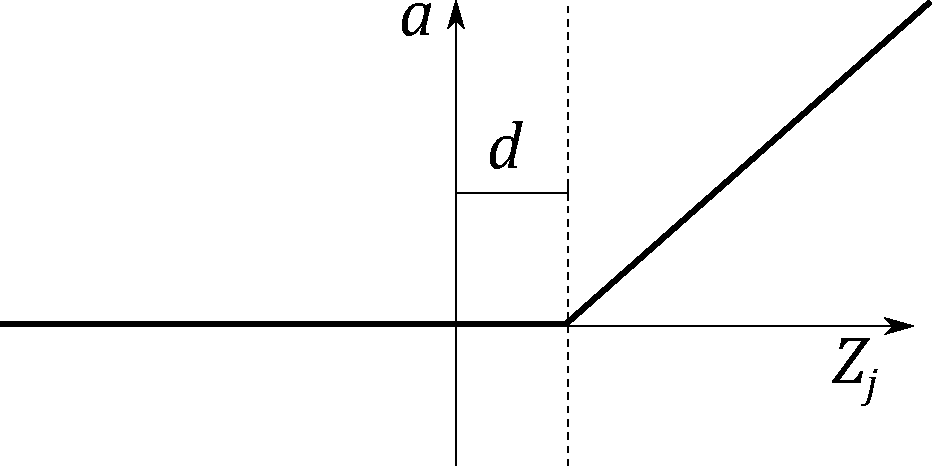
\includegraphics[width=0.5\linewidth]{images/relu.pdf}    

    \caption{In figure captions, explain what the reader is looking at: ``A schematic of the rectifying linear unit, where $a$ is the output amplitude,
    $d$ is a configurable dead-zone, and $Z_j$ is the input signal'', as well as why the reader is looking at this: 
    ``It is notable that there is no activation \emph{at all} below 0, which explains our initial results.'' 
    \textbf{Use vector image formats (.pdf) where possible}. Size figures appropriately, and do not make them over-large or too small to read.
    }

    % use the notation fig:name to cross reference a figure
    \label{fig:relu} 
\end{figure}


\begin{figure}
    \centering
    \begin{subfigure}[b]{0.45\textwidth}
        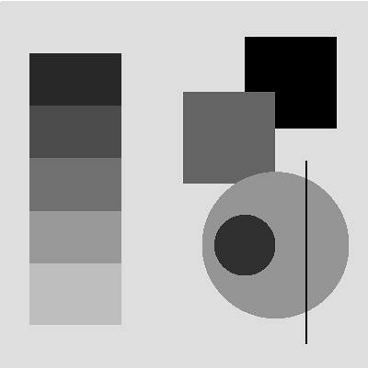
\includegraphics[width=\textwidth]{images/synthetic.png}
        \caption{Synthetic image, black on white.}
        \label{fig:syn1}
    \end{subfigure}
    ~ %add desired spacing between images, e. g. ~, \quad, \qquad, \hfill etc. 
      %(or a blank line to force the subfigure onto a new line)
    \begin{subfigure}[b]{0.45\textwidth}
        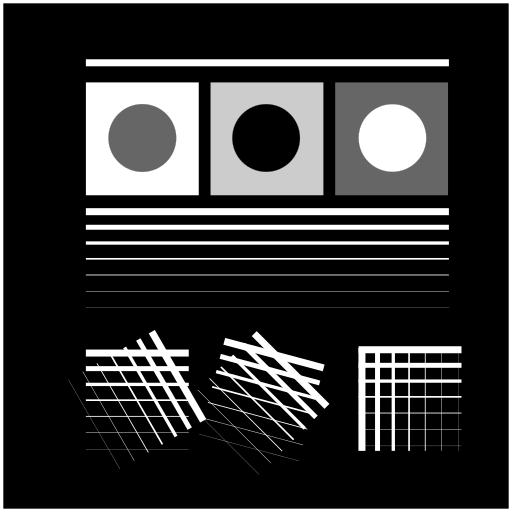
\includegraphics[width=\textwidth]{images/synthetic_2.png}
        \caption{Synthetic image, white on black.}
        \label{fig:syn2}
    \end{subfigure}
    ~ %add desired spacing between images, e. g. ~, \quad, \qquad, \hfill etc. 
    %(or a blank line to force the subfigure onto a new line)    
    \caption{Synthetic test images for edge detection algorithms. \subref{fig:syn1} shows various gray levels that require an adaptive algorithm. \subref{fig:syn2}
    shows more challenging edge detection tests that have crossing lines. Fusing these into full segments typically requires algorithms like the Hough transform.
    This is an example of using subfigures, with \texttt{subref}s in the caption.
    }\label{fig:synthetic}
\end{figure}

\clearpage

\subsection{Equations}

Equations should be typeset correctly and precisely. Make sure you get parenthesis sizing correct, and punctuate equations correctly 
(the comma is important and goes \textit{inside} the equation block). Explain any symbols used clearly if not defined earlier. 

For example, we might define:
\begin{equation}
    \hat{f}(\xi) = \frac{1}{2}\left[ \int_{-\infty}^{\infty} f(x) e^{2\pi i x \xi} \right],
\end{equation}    
where $\hat{f}(\xi)$ is the Fourier transform of the time domain signal $f(x)$.

\subsection{Algorithms}
Algorithms can be set using \texttt{algorithm2e}, as in Algorithm \ref{alg:metropolis}.

% NOTE: line ends are denoted by \; in algorithm2e
\begin{algorithm}
    \DontPrintSemicolon
    \KwData{$f_X(x)$, a probability density function returing the density at $x$.\; $\sigma$ a standard deviation specifying the spread of the proposal distribution.\;
    $x_0$, an initial starting condition.}
    \KwResult{$s=[x_1, x_2, \dots, x_n]$, $n$ samples approximately drawn from a distribution with PDF $f_X(x)$.}
    \Begin{
        $s \longleftarrow []$\;
        $p \longleftarrow f_X(x)$\;
        $i \longleftarrow 0$\;
        \While{$i < n$}
        {
            $x^\prime \longleftarrow \mathcal{N}(x, \sigma^2)$\;
            $p^\prime \longleftarrow f_X(x^\prime)$\;
            $a \longleftarrow \frac{p^\prime}{p}$\;
            $r \longleftarrow U(0,1)$\;
            \If{$r<a$}
            {
                $x \longleftarrow x^\prime$\;
                $p \longleftarrow f_X(x)$\;
                $i \longleftarrow i+1$\;
                append $x$ to $s$\;
            }
        }
    }
    
\caption{The Metropolis-Hastings MCMC algorithm for drawing samples from arbitrary probability distributions, 
specialised for normal proposal distributions $q(x^\prime|x) = \mathcal{N}(x, \sigma^2)$. The symmetry of the normal distribution means the acceptance rule takes the simplified form.}\label{alg:metropolis}
\end{algorithm}

\subsection{Tables}

If you need to include tables, like Table \ref{tab:operators}, use a tool like https://www.tablesgenerator.com/ to generate the table as it is
extremely tedious otherwise. 

\begin{table}[]
    \caption{The standard table of operators in Python, along with their functional equivalents from the \texttt{operator} package. Note that table
    captions go above the table, not below. Do not add additional rules/lines to tables. }\label{tab:operators}
    %\tt 
    \rowcolors{2}{}{gray!3}
    \begin{tabular}{@{}lll@{}}
    %\toprule
    \textbf{Operation}    & \textbf{Syntax}                & \textbf{Function}                            \\ %\midrule % optional rule for header
    Addition              & \texttt{a + b}                          & \texttt{add(a, b)}                                    \\
    Concatenation         & \texttt{seq1 + seq2}                    & \texttt{concat(seq1, seq2)}                           \\
    Containment Test      & \texttt{obj in seq}                     & \texttt{contains(seq, obj)}                           \\
    Division              & \texttt{a / b}                          & \texttt{div(a, b) }  \\
    Division              & \texttt{a / b}                          & \texttt{truediv(a, b) } \\
    Division              & \texttt{a // b}                         & \texttt{floordiv(a, b)}                               \\
    Bitwise And           & \texttt{a \& b}                         & \texttt{and\_(a, b)}                                  \\
    Bitwise Exclusive Or  & \texttt{a \textasciicircum b}           & \texttt{xor(a, b)}                                    \\
    Bitwise Inversion     & \texttt{$\sim$a}                        & \texttt{invert(a)}                                    \\
    Bitwise Or            & \texttt{a | b}                          & \texttt{or\_(a, b)}                                   \\
    Exponentiation        & \texttt{a ** b}                         & \texttt{pow(a, b)}                                    \\
    Identity              & \texttt{a is b}                         & \texttt{is\_(a, b)}                                   \\
    Identity              & \texttt{a is not b}                     & \texttt{is\_not(a, b)}                                \\
    Indexed Assignment    & \texttt{obj{[}k{]} = v}                 & \texttt{setitem(obj, k, v)}                           \\
    Indexed Deletion      & \texttt{del obj{[}k{]}}                 & \texttt{delitem(obj, k)}                              \\
    Indexing              & \texttt{obj{[}k{]}}                     & \texttt{getitem(obj, k)}                              \\
    Left Shift            & \texttt{a \textless{}\textless b}       & \texttt{lshift(a, b)}                                 \\
    Modulo                & \texttt{a \% b}                         & \texttt{mod(a, b)}                                    \\
    Multiplication        & \texttt{a * b}                          & \texttt{mul(a, b)}                                    \\
    Negation (Arithmetic) & \texttt{- a}                            & \texttt{neg(a)}                                       \\
    Negation (Logical)    & \texttt{not a}                          & \texttt{not\_(a)}                                     \\
    Positive              & \texttt{+ a}                            & \texttt{pos(a)}                                       \\
    Right Shift           & \texttt{a \textgreater{}\textgreater b} & \texttt{rshift(a, b)}                                 \\
    Sequence Repetition   & \texttt{seq * i}                        & \texttt{repeat(seq, i)}                               \\
    Slice Assignment      & \texttt{seq{[}i:j{]} = values}          & \texttt{setitem(seq, slice(i, j), values)}            \\
    Slice Deletion        & \texttt{del seq{[}i:j{]}}               & \texttt{delitem(seq, slice(i, j))}                    \\
    Slicing               & \texttt{seq{[}i:j{]}}                   & \texttt{getitem(seq, slice(i, j))}                    \\
    String Formatting     & \texttt{s \% obj}                       & \texttt{mod(s, obj)}                                  \\
    Subtraction           & \texttt{a - b}                          & \texttt{sub(a, b)}                                    \\
    Truth Test            & \texttt{obj}                            & \texttt{truth(obj)}                                   \\
    Ordering              & \texttt{a \textless b}                  & \texttt{lt(a, b)}                                     \\
    Ordering              & \texttt{a \textless{}= b}               & \texttt{le(a, b)}                                     \\
    % \bottomrule
    \end{tabular}
    \end{table}
\subsection{Code}

Avoid putting large blocks of code in the report (more than a page in one block, for example). Use syntax highlighting if possible, as in Listing \ref{lst:callahan}.

\begin{lstlisting}[language=python, float, caption={The algorithm for packing the $3\times 3$ outer-totalistic binary CA successor rule into a 
    $16\times 16\times 16\times 16$ 4 bit lookup table, running an equivalent, notionally 16-state $2\times 2$ CA.}, label=lst:callahan]
    def create_callahan_table(rule="b3s23"):
        """Generate the lookup table for the cells."""        
        s_table = np.zeros((16, 16, 16, 16), dtype=np.uint8)
        birth, survive = parse_rule(rule)

        # generate all 16 bit strings
        for iv in range(65536):
            bv = [(iv >> z) & 1 for z in range(16)]
            a, b, c, d, e, f, g, h, i, j, k, l, m, n, o, p = bv

            # compute next state of the inner 2x2
            nw = apply_rule(f, a, b, c, e, g, i, j, k)
            ne = apply_rule(g, b, c, d, f, h, j, k, l)
            sw = apply_rule(j, e, f, g, i, k, m, n, o)
            se = apply_rule(k, f, g, h, j, l, n, o, p)

            # compute the index of this 4x4
            nw_code = a | (b << 1) | (e << 2) | (f << 3)
            ne_code = c | (d << 1) | (g << 2) | (h << 3)
            sw_code = i | (j << 1) | (m << 2) | (n << 3)
            se_code = k | (l << 1) | (o << 2) | (p << 3)

            # compute the state for the 2x2
            next_code = nw | (ne << 1) | (sw << 2) | (se << 3)

            # get the 4x4 index, and write into the table
            s_table[nw_code, ne_code, sw_code, se_code] = next_code

        return s_table

\end{lstlisting}

%==================================================================================================================================
\chapter{Evaluation} 

How good is your solution?
Ask specific questions that address the general problem and answer them with evidence. Be fair and be scientific.
Compare it to other solutions for capturing reflections
Evaluation Strategy
What i did
Results
Talk about the processed graphs
What do these show

How good is your solution? How well did you solve the general problem, and what evidence do you have to support that?

\section{Guidance}
\begin{itemize}
    \item
        Ask specific questions that address the general problem.
    \item
        Answer them with precise evidence (graphs, numbers, statistical
        analysis, qualitative analysis).
    \item
        Be fair and be scientific.
    \item
        The key thing is to show that you know how to evaluate your work, not
        that your work is the most amazing product ever.
\end{itemize}

\section{Evidence}
Make sure you present your evidence well. Use appropriate visualisations, reporting techniques and statistical analysis, as appropriate.

If you visualise, follow the basic rules, as illustrated in Figure \ref{fig:boxplot}:
\begin{itemize}
\item Label everything correctly (axis, title, units).
\item Caption thoroughly.
\item Reference in text.
\item \textbf{Include appropriate display of uncertainty (e.g. error bars, Box plot)}
\item Minimize clutter.
\end{itemize}

See the file \texttt{guide\_to\_visualising.pdf} for further information and guidance.

\begin{figure}
    \centering
    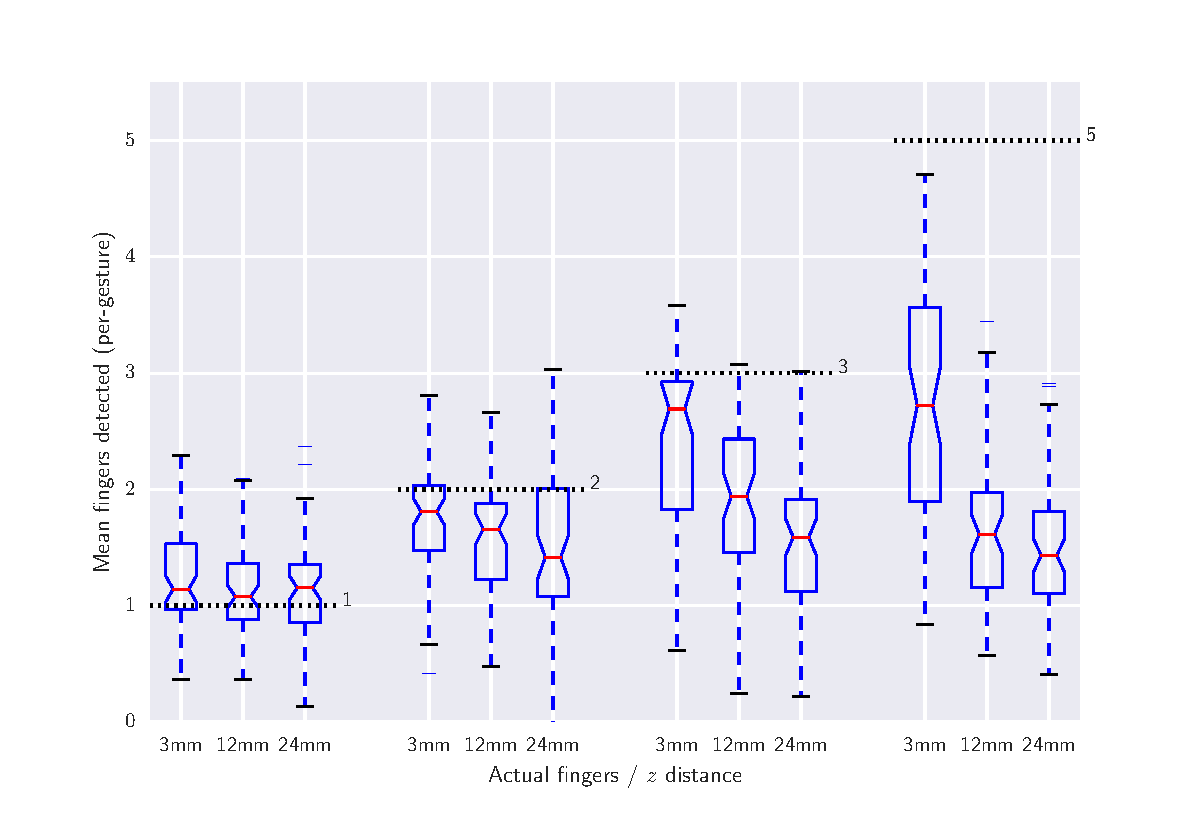
\includegraphics[width=1.0\linewidth]{images/boxplot_finger_distance.pdf}    

    \caption{Average number of fingers detected by the touch sensor at different heights above the surface, averaged over all gestures. Dashed lines indicate
    the true number of fingers present. The Box plots include bootstrapped uncertainty notches for the median. It is clear that the device is biased toward 
    undercounting fingers, particularly at higher $z$ distances.
    }

    % use the notation fig:name to cross reference a figure
    \label{fig:boxplot} 
\end{figure}


%==================================================================================================================================
\chapter{Conclusion}  

Summarise the whole project for a lazy reader who didn't read the rest (e.g. a prize-awarding committee).
Summarise briefly and fairly. Indicate what future work could be done, but remember: you won't get credit for things you haven't done.
What did i do during this project
basically go over the intro and the background and problem statement all over again
Future work
Go over how my project could be improved in the future
If i had more time on the project what i could further accomplish
Eg : could have further done tests to see whether over time users felt that they had improved on their skills, are they more aware of their skills etc
Eg : ways i could have made the app more useful, summarise the ways from the eval summaries that i could have made the app itself better
Could use a tab bar instead of the page navigation
Could use a floating '+' button instead to make a new note/recording
Personal reflections
Why did i choose swift
What did i learn by using swift that will help me in the future
Perhaps talk about how my confidence grew through using a language that was entirely new to me, gained technical skills and within myself developed the graduate attributes that i was studying
Talk about some of the difficulties i faced with it being a relatively new development method
The project was well suited to me as i enjoy HCI and the personal interaction people can have with technology and provide a better experience in their life, and about psychology aspects
Gained an interest in app development and will now further delve into this and perhaps in future create the same type of application for a webapp to see if that could provide access to a further range of people other than iOS users.  
Summarise the whole project for a lazy reader who didn't read the rest (e.g. a prize-awarding committee).


\section{Guidance}
\begin{itemize}
    \item
        Summarise briefly and fairly.
    \item
        You should be addressing the general problem you introduced in the
        Introduction.        
    \item
        Include summary of concrete results (``the new compiler ran 2x
        faster'')
    \item
        Indicate what future work could be done, but remember: \textbf{you
        won't get credit for things you haven't done}.
\end{itemize}

%==================================================================================================================================
%
% 
%==================================================================================================================================
%  APPENDICES  

\begin{appendices}

\chapter{Appendices}

Typical inclusions in the appendices are:

\begin{itemize}
\item
  Copies of ethics approvals (required if obtained)
\item
  Copies of questionnaires etc. used to gather data from subjects.
\item
  Extensive tables or figures that are too bulky to fit in the main body of
  the report, particularly ones that are repetitive and summarised in the body.

\item Outline of the source code (e.g. directory structure), or other architecture documentation like class diagrams.

\item User manuals, and any guides to starting/running the software.

\end{itemize}

\textbf{Don't include your source code in the appendices}. It will be
submitted separately.

\end{appendices}

%==================================================================================================================================
%   BIBLIOGRAPHY   

% The bibliography style is abbrvnat
% The bibliography always appears last, after the appendices.

\bibliographystyle{abbrvnat}

\bibliography{l4proj}

\end{document}
